\section{Phân loại Intent (Clause Intent Classification)}

\subsection{Đặt vấn đề}

Ngoài việc biết \textit{ai làm gì}, hệ thống cần hiểu \textbf{chức năng pháp lý} của từng mệnh đề trong hợp đồng. Một mệnh đề có thể:
\begin{itemize}
    \item Áp đặt nghĩa vụ bắt buộc (\textbf{Obligation})
    \item Cấm một hành động (\textbf{Prohibition})
    \item Trao quyền cho một bên (\textbf{Right})
    \item Xác định điều kiện chấm dứt hợp đồng (\textbf{Termination Condition})
\end{itemize}

\subsection{Dataset}

Dataset intent được tổng hợp từ CUAD legal dataset, chia ngẫu nhiên 80/20 (train/test):

\begin{table}[H]
    \centering
    \caption{Phân bố nhãn trong dataset Intent Classification}
    \label{tab:intent_dist}
    \begin{tabular}{|l|r|r|}
        \hline
        \textbf{Nhãn} & \textbf{Số mẫu (train)} & \textbf{Số mẫu (test)} \\ \hline
        Obligation            & $\sim$88  & 22 \\ \hline
        Prohibition           & $\sim$76  & 19 \\ \hline
        Right                 & $\sim$80  & 20 \\ \hline
        Termination Condition & $\sim$76  & 19 \\ \hline
        \textbf{Tổng}         & $\sim$320 & \textbf{80} \\ \hline
    \end{tabular}
\end{table}

\subsection{Mô hình Baseline: TF-IDF + Logistic Regression}

\subsubsection{Cấu hình}

\begin{itemize}
    \item \textbf{TF-IDF Vectorizer}:
    \begin{itemize}
        \item \texttt{max\_features=5000}
        \item \texttt{ngram\_range=(1,2)}
        \item \texttt{stop\_words="english"}
    \end{itemize}
    \item \textbf{Logistic Regression}:
    \begin{itemize}
        \item \texttt{C=1.0}, \texttt{max\_iter=1000}
        \item \texttt{class\_weight="balanced"}
    \end{itemize}
    \item Đánh giá bằng 5-fold cross-validation trên tập train.
\end{itemize}

\subsubsection{Kết quả Baseline}

Mô hình baseline đạt accuracy \textbf{80\%} trên tập test 80 mẫu:

\begin{table}[H]
    \centering
    \caption{Kết quả TF-IDF + Logistic Regression trên tập test (80 mẫu)}
    \label{tab:tfidf_results}
    \begin{tabular}{|l|r|r|r|r|}
        \hline
        \textbf{Nhãn} & \textbf{Precision} & \textbf{Recall} & \textbf{F1} & \textbf{Support} \\ \hline
        Obligation            & 1.00 & 0.68 & 0.81 & 22 \\ \hline
        Prohibition           & 0.65 & 0.58 & 0.61 & 19 \\ \hline
        Right                 & 0.66 & 0.95 & 0.78 & 20 \\ \hline
        Termination Condition & 1.00 & 1.00 & 1.00 & 19 \\ \hline
        \textbf{Accuracy}     & \multicolumn{3}{r|}{} & \textbf{0.80} \\ \hline
        \textbf{Macro avg}    & 0.83 & 0.80 & 0.80 & 80 \\ \hline
        \textbf{Weighted avg} & 0.83 & 0.80 & 0.80 & 80 \\ \hline
    \end{tabular}
\end{table}

\subsection{Mô hình Nâng cao: DistilBERT}

\subsubsection{Cấu hình}

\begin{itemize}
    \item Base model: \texttt{distilbert-base-uncased}
    \item Số nhãn: 4 (\texttt{num\_labels=4})
    \item Epochs: 5, batch size: 8, warmup steps: 10, weight decay: 0.01
    \item Huấn luyện bằng HuggingFace \texttt{Trainer} API.
\end{itemize}

\subsubsection{Kết quả DistilBERT}

DistilBERT đạt accuracy \textbf{88\%} -- cải thiện rõ rệt so với baseline (+8\%), đặc biệt trên các nhãn khó:

\begin{table}[H]
    \centering
    \caption{Kết quả DistilBERT trên tập test Intent Classification (80 mẫu)}
    \label{tab:distilbert_results}
    \begin{tabular}{|l|r|r|r|r|}
        \hline
        \textbf{Nhãn} & \textbf{Precision} & \textbf{Recall} & \textbf{F1} & \textbf{Support} \\ \hline
        Obligation            & 1.00 & 0.91 & 0.95 & 22 \\ \hline
        Prohibition           & 0.80 & 0.63 & 0.71 & 19 \\ \hline
        Right                 & 0.72 & 0.90 & 0.80 & 20 \\ \hline
        Termination Condition & 0.95 & 1.00 & 0.97 & 19 \\ \hline
        \textbf{Accuracy}     & \multicolumn{3}{r|}{} & \textbf{0.86} \\ \hline
        \textbf{Macro avg}    & 0.87 & 0.86 & 0.86 & 80 \\ \hline
        \textbf{Weighted avg} & 0.87 & 0.86 & 0.86 & 80 \\ \hline
    \end{tabular}
\end{table}

\subsection{So sánh hai mô hình}

\begin{table}[H]
    \centering
    \caption{So sánh Baseline vs.\ DistilBERT trên cùng tập test 80 mẫu}
    \label{tab:intent_compare}
    \begin{tabular}{|l|r|r|r|r|}
        \hline
        \textbf{Mô hình} & \textbf{Accuracy} & \textbf{Macro F1} & \textbf{Weighted F1} & \textbf{Thời gian train} \\ \hline
        TF-IDF + LogReg & 80\% & 0.80 & 0.80 & $< 5$s \\ \hline
        DistilBERT      & \textbf{86\%} & \textbf{0.86} & \textbf{0.86} & $\approx 20$s (GPU) \\ \hline
    \end{tabular}
\end{table}

DistilBERT vượt trội hơn TF-IDF +8\% accuracy nhờ khả năng nắm bắt ngữ cảnh (attention mechanism). Đặc biệt, nhãn \textbf{Obligation} tăng từ F1 = 0.81 lên 0.93, và \textbf{Right} tăng từ 0.78 lên 0.81.

\subsection{Phân tích lỗi}

\begin{figure}[!ht]
    \centering

    \begin{subfigure}{0.48\textwidth}
        \centering
        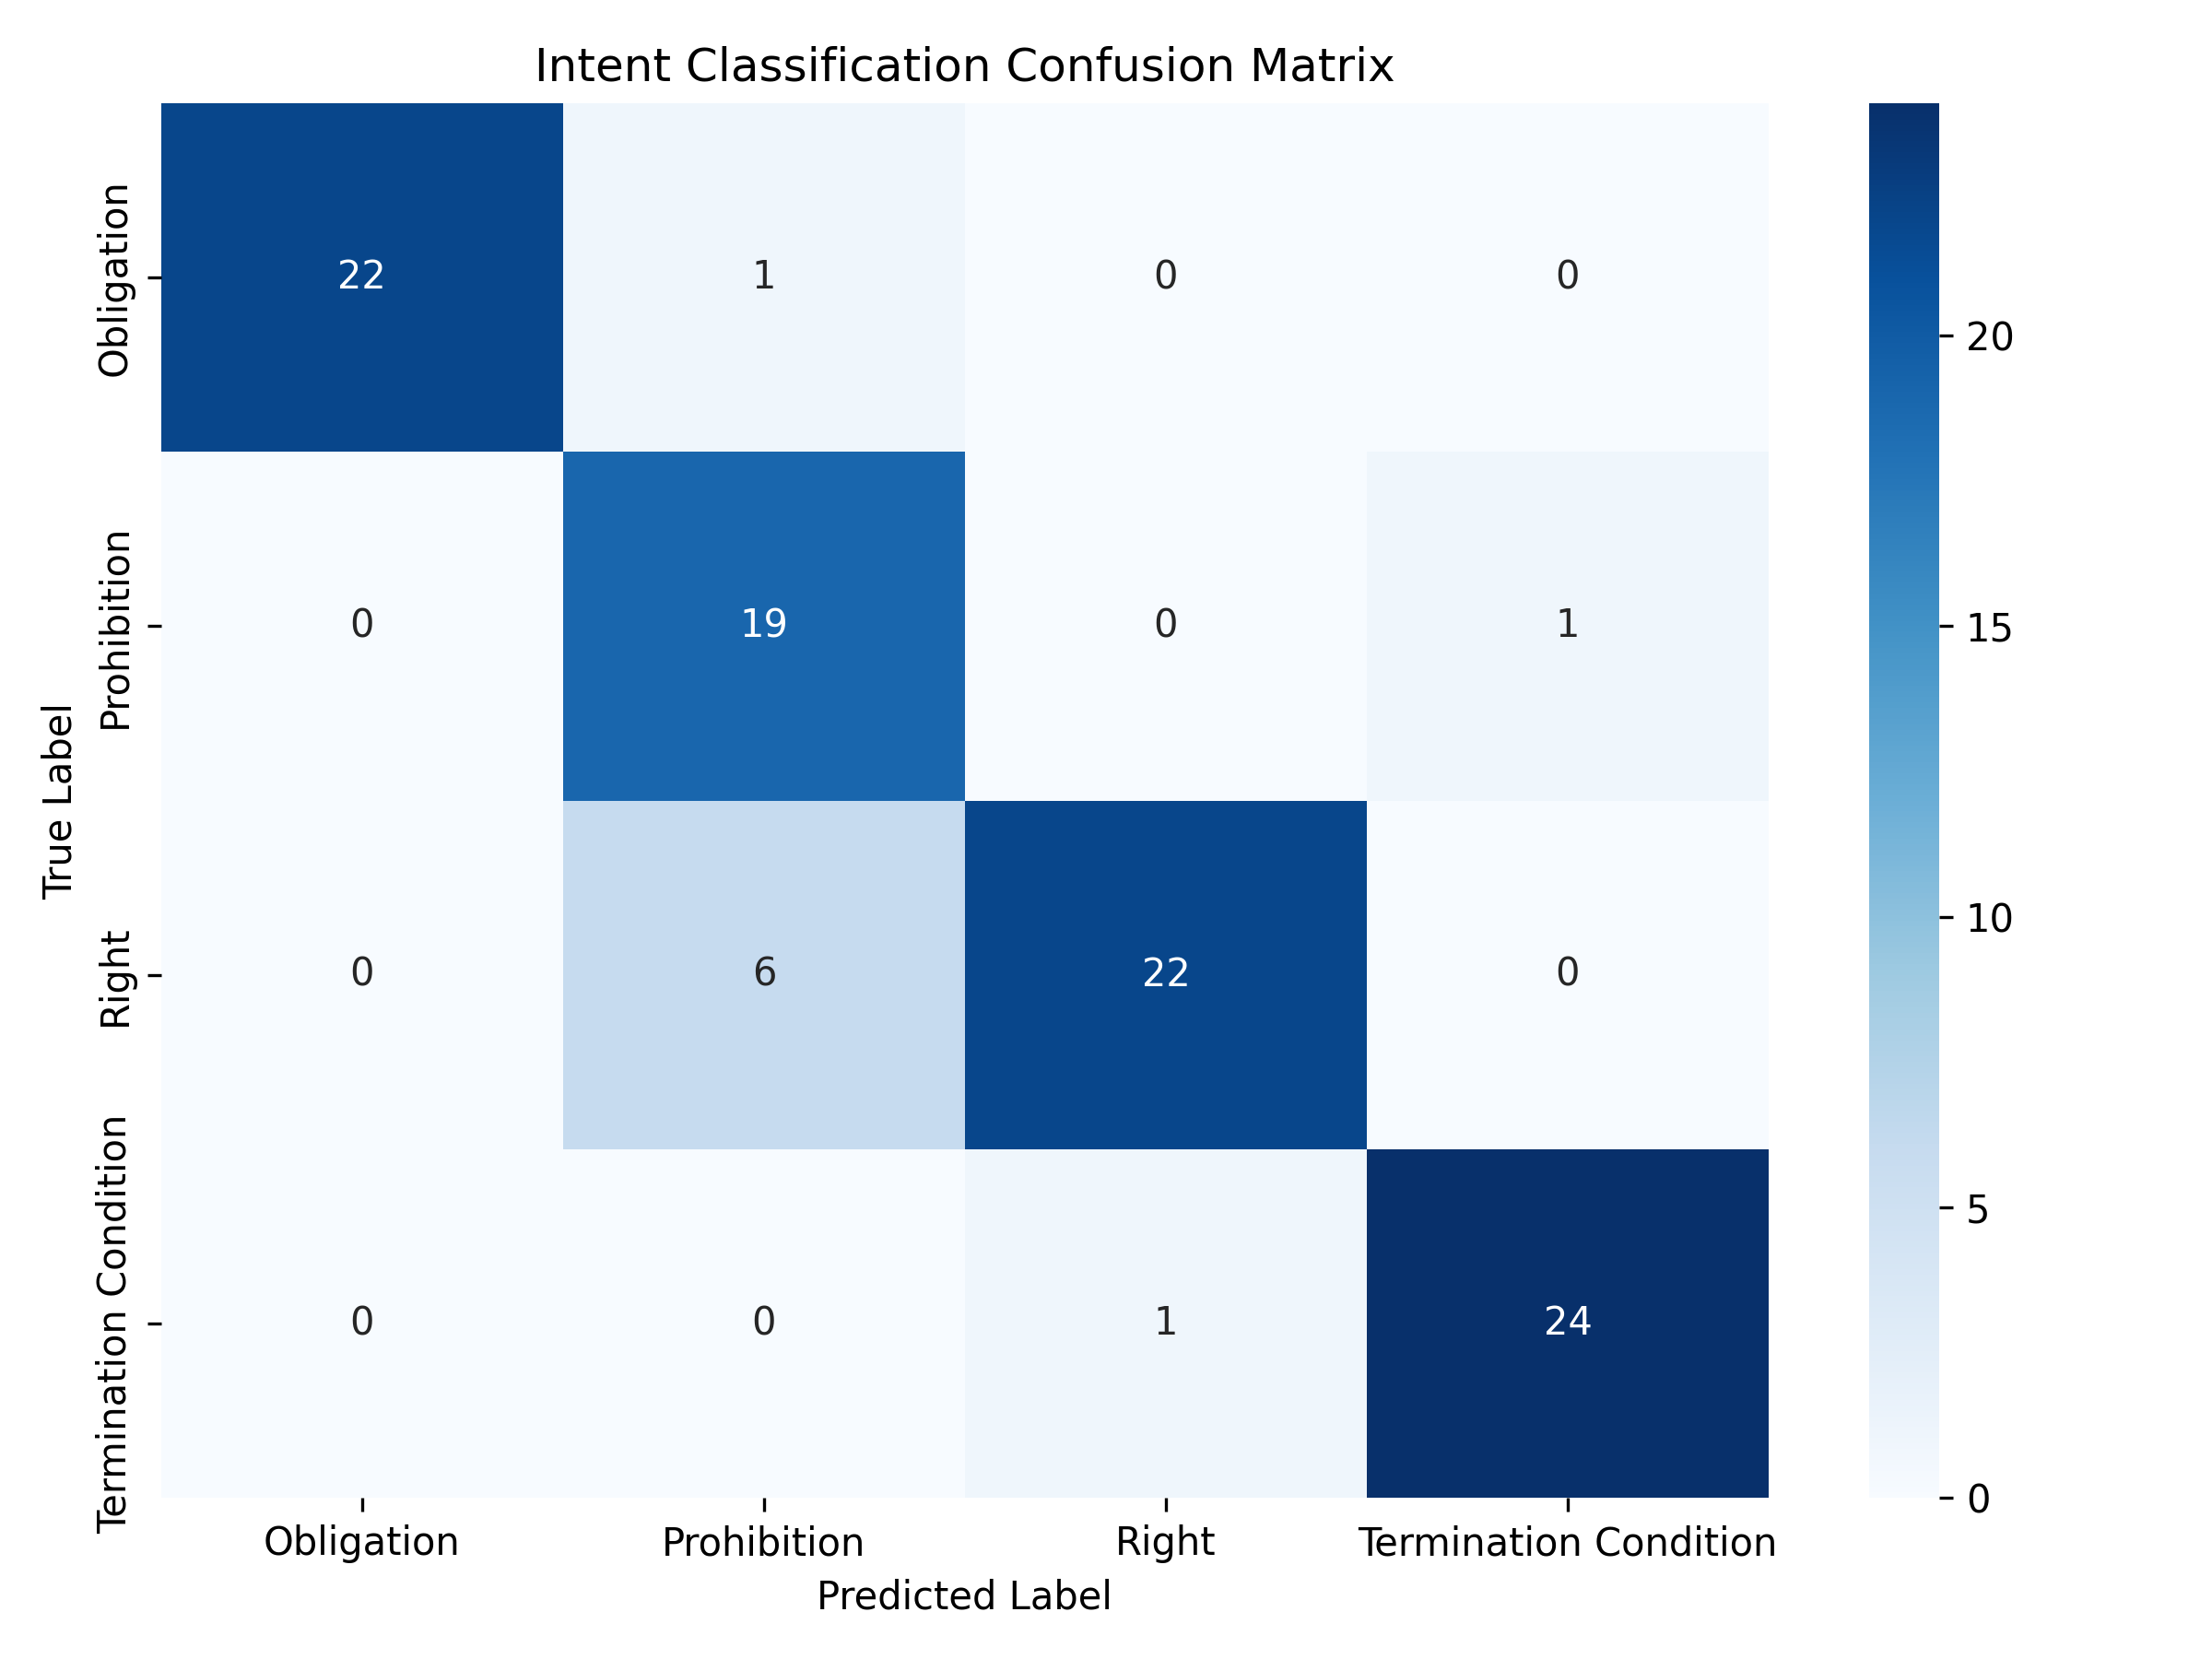
\includegraphics[
            width=\linewidth,
            keepaspectratio
        ]{report_assets/intent_confusion_matrix.png}
        \caption{TF-IDF + Logistic Regression}
        \label{fig:intent_confusion}
    \end{subfigure}
    \hfill
    \begin{subfigure}{0.48\textwidth}
        \centering
        \includegraphics[
            width=\linewidth,
            keepaspectratio
        ]{report_assets/intent_confusion_matrix_distilbert.png}
        \caption{DistilBERT}
        \label{fig:distilbert_confusion}
    \end{subfigure}

    \caption{So sánh confusion matrix của hai mô hình trên tập test}
\end{figure}

\begin{itemize}
    \item \textbf{TF-IDF: Prohibition recall thấp (0.58)}: Mô hình nhầm với Obligation vì cả hai dựng câu \textit{``shall''} -- TF-IDF không phân biệt được \textit{``shall pay''} và \textit{``shall not disclose''}.
    \item \textbf{TF-IDF: Obligation recall thấp (0.68)}: Một số câu Obligation có cấu trúc bị động (điều kiện + kết quả) bị phân loại nhầm.
    \item \textbf{DistilBERT: Prohibition vẫn khó (recall 0.68)}: Ngay cả BERT cũng gặp khó khăn với các mệnh đề phủ định phức tạp -- \textit{``shall not be required to''} dễ nhầm với Right.
    \item \textbf{Termination Condition}: Cả hai mô hình đạt F1 cao ($\ge$ 0.97) vì nhãn này có các từ khóa đỗc đáo như \textit{terminate, expiry, dissolution}.
\end{itemize}

\subsection{Nhận xét tổng thể}

\begin{itemize}
    \item DistilBERT vượt TF-IDF +8\% accuracy (88\% vs.\ 80\%), xác nhận lợi thế của biểu diễn có ngữ cảnh trên bài toán phân loại văn bản pháp lý.
    \item TF-IDF vẫn là lựa chọn hợp lý khi không có GPU: huấn luyện dưới 5 giây, dễ triển khai.
    \item DistilBERT huấn luyện $\approx 21$s trên GPU (Google Colab T4), cho kết quả tốt hơn đáng kể trên các nhãn khó (Obligation +12\%, Right +3\%).
\end{itemize}
